% USEFUL LINKS:
% -------------
%
% - UiO LaTeX guides:          https://www.mn.uio.no/ifi/tjenester/it/hjelp/latex/
% - Mathematics:               https://en.wikibooks.org/wiki/LaTeX/Mathematics
% - Physics:                   https://ctan.uib.no/macros/latex/contrib/physics/physics.pdf
% - Basics of Tikz:            https://en.wikibooks.org/wiki/LaTeX/PGF/Tikz
% - All the colors!            https://en.wikibooks.org/wiki/LaTeX/Colors
% - How to make tables:        https://en.wikibooks.org/wiki/LaTeX/Tables
% - Code listing styles:       https://en.wikibooks.org/wiki/LaTeX/Source_Code_Listings
% - \includegraphics           https://en.wikibooks.org/wiki/LaTeX/Importing_Graphics
% - Learn more about figures:  https://en.wikibooks.org/wiki/LaTeX/Floats,_Figures_and_Captions
% - Automagic bibliography:    https://en.wikibooks.org/wiki/LaTeX/Bibliography_Management  (this one is kinda difficult the first time)
%
%                              (This document is of class "revtex4-1", the REVTeX Guide explains how the class works)
%   REVTeX Guide:              http://www.physics.csbsju.edu/370/papers/Journal_Style_Manuals/auguide4-1.pdf
%
%
% COMPILING THE .pdf FILE IN THE LINUX TERMINAL
% ---------------------------------------------
%
% [terminal]$ pdflatex report_example.tex
%
% Run the command twice, always.
%
% When using references, footnotes, etc. you should run the following chain of commands:
%
% [terminal]$ pdflatex report_example.tex
% [terminal]$ bibtex report_example
% [terminal]$ pdflatex report_example.tex
% [terminal]$ pdflatex report_example.tex
%
% This series of commands can of course be gathered into a single-line command:
% [terminal]$ pdflatex report_example.tex && bibtex report_example.aux && pdflatex report_example.tex && pdflatex report_example.tex
%
% ----------------------------------------------------



% \documentclass[english,notitlepage,reprint,nofootinbib]{revtex4-2}  % defines the basic parameters of the document
\documentclass[english,notitlepage,reprint,nofootinbib]{revtex4-2}  % defines the basic parameters of the document
% If you want a single-column, remove "reprint"

% Allows special characters (including æøå)
\usepackage[utf8]{inputenc}
% \usepackage[english]{babel}

% Note that you may need to download some of these packages manually, it depends on your setup.
% It may be usefult to download TeXMaker, because it includes a large library of the most common packages.

\usepackage{physics,amssymb}  % mathematical symbols (physics imports amsmath)
\include{amsmath}
\usepackage{graphicx}         % include graphics such as plots
\usepackage{xcolor}           % set colors
\usepackage{hyperref}         % automagic cross-referencing
\usepackage{listings}         % display code
\usepackage{subfigure}        % imports a lot of cool and useful figure commands
% \usepackage{float}
%\usepackage[section]{placeins}
\usepackage{algorithm}
\usepackage[noend]{algpseudocode}
\usepackage{subfigure}
\usepackage{tikz}
\usetikzlibrary{quantikz}
% defines the color of hyperref objects
% Blending two colors:  blue!80!black  =  80% blue and 20% black
\hypersetup{ % this is just my personal choice, feel free to change things
    colorlinks,
    linkcolor={red!50!black},
    citecolor={blue!50!black},
    urlcolor={blue!80!black}}


% ===========================================


\begin{document}

\title{Study of Ca+ Ions in a Penning Trap}  % self-explanatory
\author{Émilie Valle, Joseph Ayman}       % self-explanatory
\date{\today}                             % self-explanatory
\noaffiliation                            % ignore this, but keep it.

%This is how we create an abstract section.
\begin{abstract}
     In this report, we investigate the behavior of Ca+ ions confined in a Penning trap. We develop a numerical simulation to model the motion of charged particles under the influence of static and time-dependent electromagnetic fields. Our study focuses on understanding the dynamics of single and multiple particles, the effects of particle interactions, and the resonance phenomena in the trap.
    
\end{abstract}
\maketitle


% ===========================================
\section{Introduction}\label{sec:introduction}
In modern experimental physics, the ability to precisely control and manipulate individual charged particles is crucial for a wide range of applications, from mass spectrometry to antimatter research. One of the most important tools for achieving this control is the \textbf{Penning trap}, a device that uses a combination of static electric and magnetic fields to confine charged particles in a well-defined region of space. Despite its relative simplicity, the Penning trap has become an indispensable instrument in experimental physics, playing a vital role in experiments at CERN such as ALPHA, AEgIS, and BASE, particularly in antimatter research.

The fundamental principle behind the Penning trap, first developed by Hans Georg Dehmelt (who later won the 1989 Nobel Prize in Physics for this work)\footnote{\url{https://en.wikipedia.org/wiki/Penning_trap}}, involves the clever combination of a quadrupole electric field for axial confinement and a uniform magnetic field for radial confinement. The electric field creates a potential well that traps particles along the axis of the device, while the magnetic field induces a circular motion that prevents particles from escaping radially. This configuration allows for the precise manipulation and study of charged particles for extended periods.

In this project, we develop a comprehensive numerical simulation of a Penning trap to study the dynamics of charged calcium ions (Ca$^+$) under various conditions. Our simulation implements both single-particle and many-particle scenarios, allowing us to investigate not only the fundamental behavior of individual ions but also the complex interactions that arise when multiple particles are present. We employ two numerical methods -- the Forward Euler method and the fourth-order Runge-Kutta method -- to solve the equations of motion, and we compare their accuracy and efficiency against analytical solutions where available.

The simulation explores several key aspects of the Penning trap:
\begin{itemize}
\item The motion of single particles, comparing numerical results with analytical solutions
\item The dynamics of multiple particles, including the effects of Coulomb interactions
\item The impact of time-varying electric fields on particle confinement
\item The resonant frequencies that can lead to particle ejection from the trap
\end{itemize}

We have implemented our simulation in C++ using the Armadillo library for efficient numerical computations, following an object-oriented approach that separates the particle and trap physics into distinct classes. This design allows for flexible testing of different configurations and easy extension to more complex scenarios.

The report is organized as follows: In Section \ref{sec:methods}, we present the theoretical framework, deriving the equations of motion for particles in the trap and discussing the analytical solutions for the single-particle case. In Section \ref{sec:results_and_discussion}, we present our results, comparing the numerical methods' accuracy and exploring the behavior of multiple interacting particles. Finally, Section \ref{sec:conclusion} summarizes our findings and discusses potential applications and extensions of this work.

All code developed for this report is available via a GitHub repository.\footnote{\url{https://github.uio.no/josefam/FYS3150/tree/main/project3}}
% ===========================================
\section{Methods}\label{sec:methods}

\subsection{Physical Theory and Analytical Solutions}
The Penning trap confines charged particles using a combination of static electric and magnetic fields. The total force $\mathbf{F}$ acting on a particle with charge $q$ and velocity $\mathbf{v}$ is given by the Lorentz force:
\begin{equation}
\mathbf{F} = q\mathbf{E} + q\mathbf{v}\times \mathbf{B},
\end{equation}
where $\mathbf{E}$ is the electric field and $\mathbf{B}$ is the magnetic field. From Newton's second law:
\begin{equation}
m\ddot{\mathbf{r}} = \mathbf{F},
\end{equation}
In our ideal Penning trap, the electric field is derived from the potential:
\begin{equation}
V(x, y, z) = \frac{V_0}{2d^2}(2z^2 - x^2 - y^2),
\end{equation}
giving:
\begin{equation}
\mathbf{E} = -\nabla V = \frac{V_0}{d^2}(x\hat{e}_x + y\hat{e}_y - 2z\hat{e}_z).
\end{equation}
The magnetic field is uniform along the z-axis:
\begin{equation}
\mathbf{B} = B_0\hat{e}_z.
\end{equation}
\subsubsection{Single-Particle Motion}
For a single particle, combining Newton's law with the Lorentz force yields three coupled differential equations:
\begin{align}
\ddot{x} - \omega_0 \dot{y} - \frac{1}{2}\omega_z^2 x &= 0, \
\ddot{y} + \omega_0 \dot{x} - \frac{1}{2}\omega_z^2 y &= 0, \
\ddot{z} + \omega_z^2 z &= 0,
\end{align}
where we define the characteristic frequencies:
\begin{equation}
\omega_0 \equiv \frac{qB_0}{m}, \quad \omega_z^2 \equiv \frac{2qV_0}{md^2}.
\end{equation}
The equation for $z$ is a simple harmonic oscillator with general solution:
\begin{equation}
z(t) = A\cos(\omega_z t + \phi),
\end{equation}
where $A$ and $\phi$ are determined by initial conditions.
\subsubsection{Complex Representation}
The coupled equations for $x$ and $y$ can be elegantly combined by introducing a complex function $f(t) = x(t) + iy(t)$. Taking the second derivative:
\begin{equation}
\ddot{f} = \ddot{x} + i\ddot{y},
\end{equation}
and substituting from the original equations:
\begin{equation}
\ddot{f} = \omega_0(\dot{y} - i\dot{x}) + \frac{1}{2}\omega_z^2(x + iy).
\end{equation}
Using $i\dot{f} = i\dot{x} - \dot{y}$, we obtain:
\begin{equation}
\ddot{f} + i\omega_0\dot{f} - \frac{1}{2}\omega_z^2f = 0.
\end{equation}
The general solution to this equation is:
\begin{equation}
f(t) = A_+ e^{-i(\omega_+ t + \phi_+)} + A_- e^{-i(\omega_- t + \phi_-)},
\end{equation}
where:
\begin{equation}
\omega_\pm = \frac{\omega_0 \pm \sqrt{\omega_0^2 - 2\omega_z^2}}{2}.
\end{equation}
\subsubsection{Stability Conditions}
For the solution to remain bounded (i.e., $|f(t)| < \infty$ as $t\to\infty$), $\omega_\pm$ must be real, requiring:
\begin{equation}
\omega_0^2 > 2\omega_z^2.
\end{equation}
In terms of the trap parameters, this gives:
\begin{equation}
\frac{q}{m} > \frac{4V_0}{B_0d^2}.
\end{equation}
The particle's radial bounds in the xy-plane are:
\begin{equation}
R_+ = A_+ + A_-, \quad R_- = |A_+ - A_-|,
\end{equation}
which can be proven by considering $|f(t)| = \sqrt{f(t)f^*(t)}$ and finding its extrema.
\subsubsection{Multiple-Particle Dynamics}
For $n$ particles with charges ${q_i}$ and masses ${m_i}$, the equations of motion include Coulomb interactions:
\begin{equation}
m_i\ddot{\mathbf{r}}_i = q_i\mathbf{E} + q_i\mathbf{v}i\times \mathbf{B} + k_e q_i\sum{j\neq i}q_j \frac{\mathbf{r}_i-\mathbf{r}_j}{|\mathbf{r}_i - \mathbf{r}_j|^3},
\end{equation}
where $k_e$ is Coulomb's constant and the sum represents the total Coulomb force on particle $i$ from all other particles.

\subsection{Numerical Methods}

\subsubsection{Forward Euler Method}

To solve these equations numerically, we first implement the Forward Euler method. For a system of first-order differential equations $\dot{\mathbf{y}} = \mathbf{f}(t, \mathbf{y})$, the Forward Euler method advances the solution from time $t_n$ to $t_{n+1}$ using:

\begin{equation}
    \mathbf{y}_{n+1} = \mathbf{y}_n + h\mathbf{f}(t_n, \mathbf{y}_n),
\end{equation}

where $h$ is the time step.

\subsubsection{Fourth-Order Runge-Kutta Method}

For improved accuracy, we also implement the fourth-order Runge-Kutta method (RK4). For the same system, RK4 advances the solution using:

\begin{align}
    \mathbf{k}_1 &= h\mathbf{f}(t_n, \mathbf{y}_n), \\
    \mathbf{k}_2 &= h\mathbf{f}(t_n + \frac{h}{2}, \mathbf{y}_n + \frac{\mathbf{k}_1}{2}), \\
    \mathbf{k}_3 &= h\mathbf{f}(t_n + \frac{h}{2}, \mathbf{y}_n + \frac{\mathbf{k}_2}{2}), \\
    \mathbf{k}_4 &= h\mathbf{f}(t_n + h, \mathbf{y}_n + \mathbf{k}_3),
\end{align}

with the final update:

\begin{equation}
    \mathbf{y}_{n+1} = \mathbf{y}_n + \frac{1}{6}(\mathbf{k}_1 + 2\mathbf{k}_2 + 2\mathbf{k}_3 + \mathbf{k}_4).
\end{equation}

\subsection{Implementation Details}

Our implementation uses two main classes:

\begin{itemize}
    \item \texttt{Particle}: Stores and manages particle properties (position, velocity, charge, mass)
    \item \texttt{PenningTrap}: Handles the trap configuration and particle interactions
\end{itemize}

We use the following units throughout our implementation:
\begin{itemize}
    \item Length: micrometres ($\mathrm{\mu m}$)
    \item Time: microseconds ($\mathrm{\mu s}$)
    \item Mass: atomic mass unit ($\mathrm{u}$)
    \item Charge: elementary charge ($\mathrm{e}$)
\end{itemize}

The default trap parameters are:
\begin{itemize}
    \item $B_0 = 9.65 \times 10^1 \frac{\mathrm{u}}{\mathrm{\mu s\, e}}$
    \item $V_0 = 2.41 \times 10^6 \frac{\mathrm{u\, \mu m^2}}{\mathrm{\mu s^2\, e}}$
    \item $d = 500\,\mathrm{\mu m}$
\end{itemize}

For the resonance studies, we modify the electric potential to include a time-dependent term:

\begin{equation}
    V_0 \rightarrow V_0(1 + f\cos(\omega_V t)),
\end{equation}

where $f$ is the relative amplitude and $\omega_V$ is the driving frequency.

\subsection{Tools}
The implementation of our Penning trap simulation was developed using several computational tools and libraries. The core simulation was written in C++, utilizing the Armadillo library for efficient linear algebra operations and vector calculations. We chose C++ for its performance advantages in numerical computations and object-oriented programming capabilities, while Armadillo provided optimized matrix operations essential for particle trajectory calculations.
For data visualization and analysis, we employed Python with key libraries:
\begin{itemize}
\item \texttt{matplotlib} for generating plots and visualizing particle trajectories
\item \texttt{numpy} for numerical operations and data handling
\end{itemize}
The development was conducted using Visual Studio Code as our primary text editor, chosen for its integrated debugging capabilities and extensive language support. For version control and code organization, we utilized Git through GitHub's services.
ChatGPT was employed during the writing phase for proofreading and grammatical improvements of our scientific report. The report was written and compiled using Overleaf, an online LaTeX editor, with the \texttt{RevTeX} document class, which is commonly used for physics publications.
% ===========================================

\section{Results and discussion}\label{sec:results_and_discussion}

\subsection{Single Particle Dynamics}

We begin our analysis by examining the motion of a single Ca$^+$ ion in the Penning trap, comparing our numerical solutions with the analytical prediction. Figure \ref{fig:single_particle} shows the particle's trajectory in the $z$-direction over a period of 50 $\mu$s, computed using both the Forward Euler and fourth-order Runge-Kutta (RK4) methods.

\begin{figure}[h!]
    \centering
    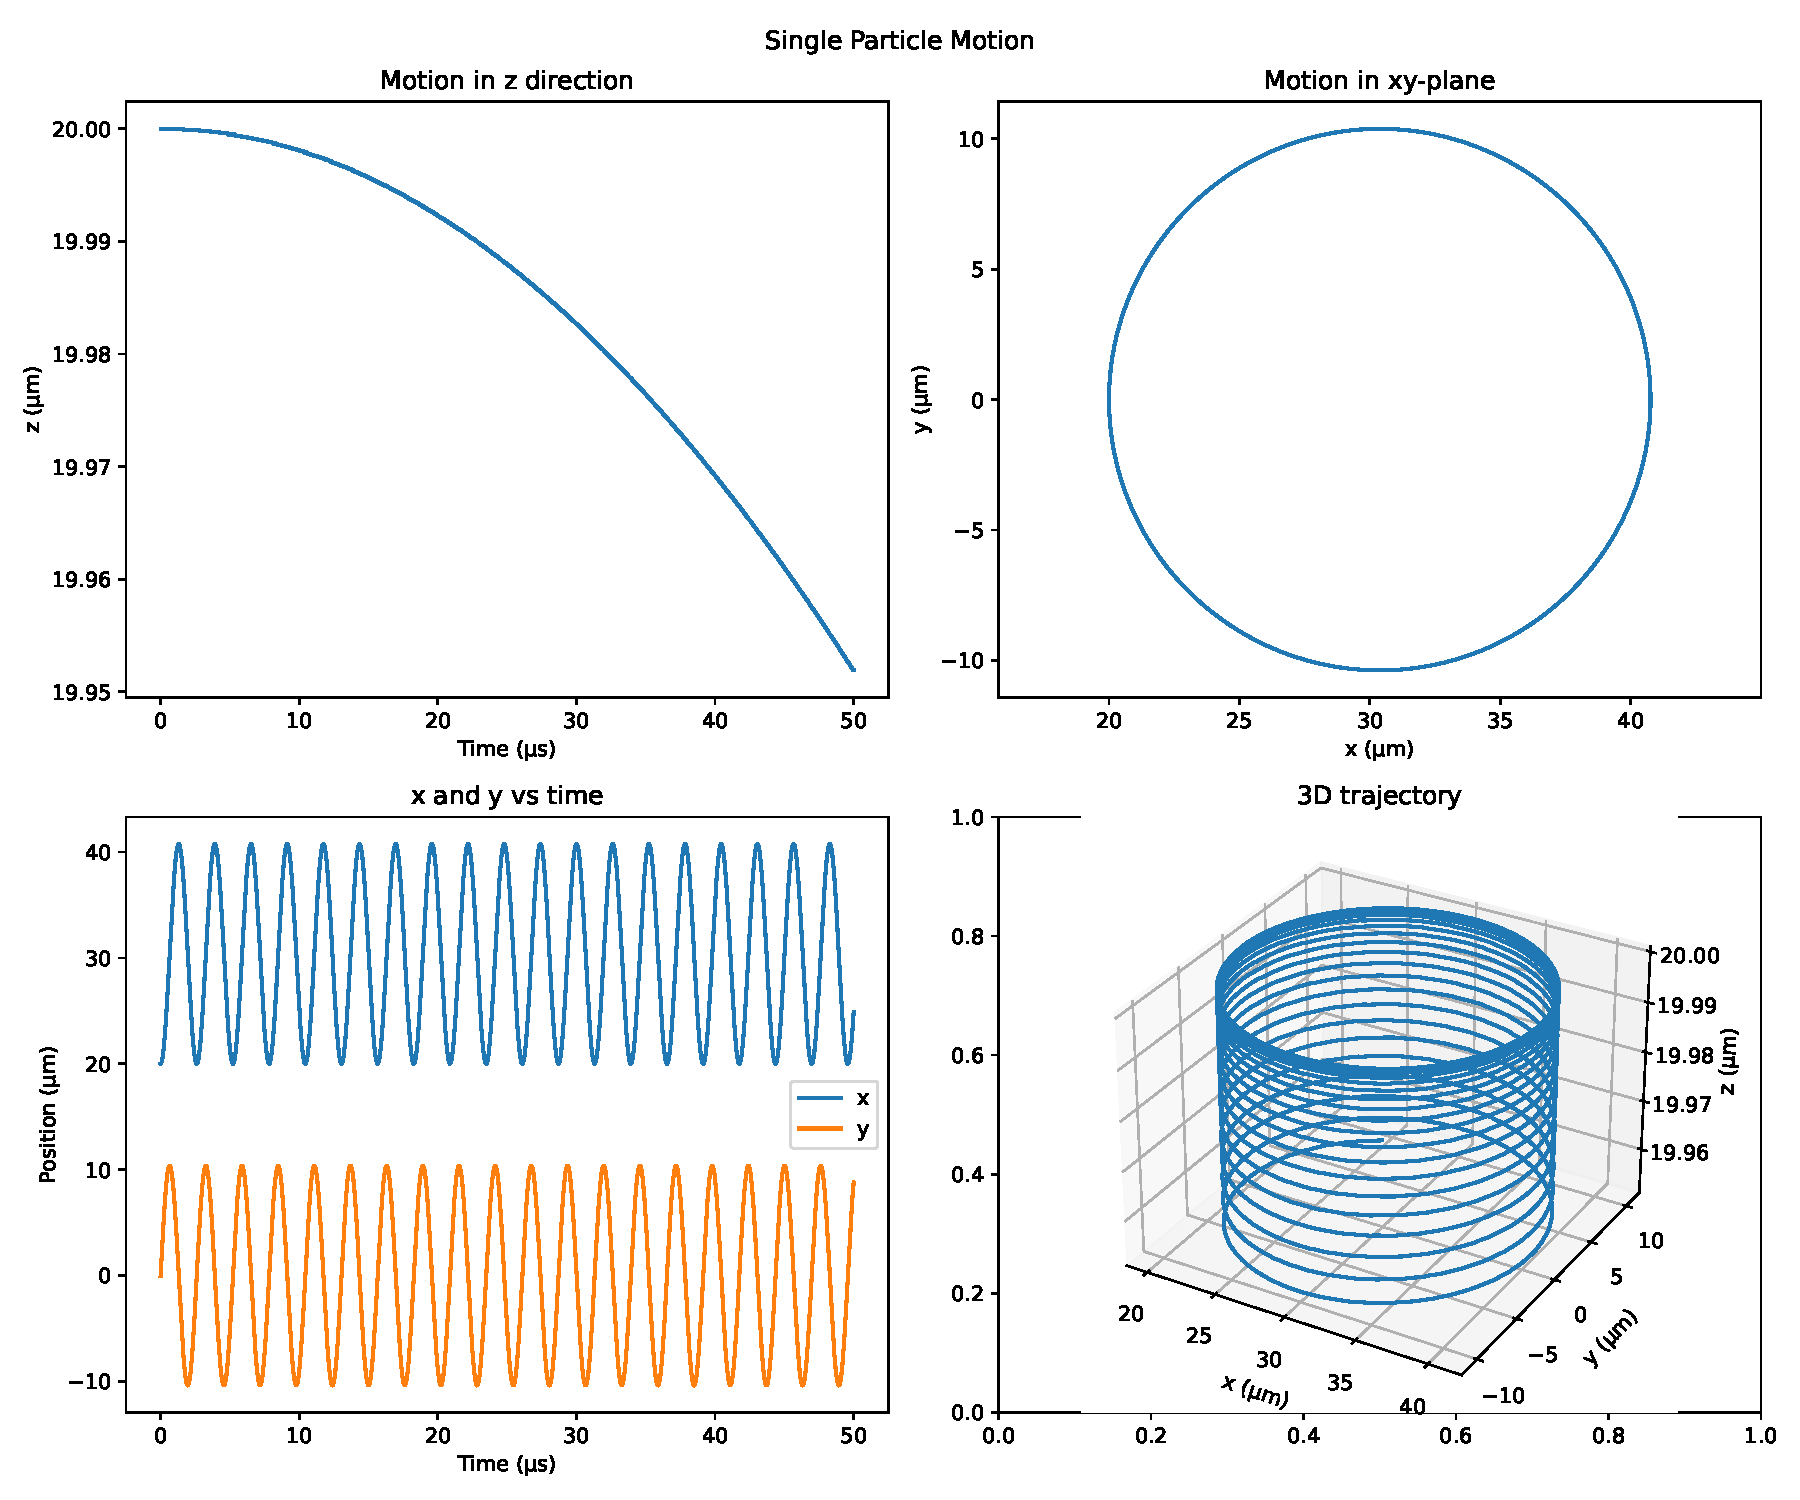
\includegraphics[width=0.48\textwidth]{build/figures/single_particle_motion.pdf}
    \caption{Motion of a single Ca$^+$ ion in the Penning trap. The left panel shows the oscillatory motion in the $z$-direction, while the right panel displays the particle's trajectory in the $xy$-plane. Initial conditions: $\mathbf{r}_0 = (20,0,20)$ $\mu$m, $\mathbf{v}_0 = (0,25,0)$ $\mu$m/$\mu$s.}
    \label{fig:single_particle}
\end{figure}

The particle exhibits stable oscillatory motion in the $z$-direction, with the RK4 method closely matching the analytical solution. The Forward Euler method, while capturing the general behavior, shows noticeable deviations from the exact solution, particularly over longer time periods. This difference in accuracy is expected, given the first-order nature of the Forward Euler method compared to the fourth-order accuracy of RK4.

\subsection{Two-Particle System}

The dynamics become more complex when we introduce a second particle into the trap. Figure \ref{fig:two_particles} compares the trajectories of two particles with and without Coulomb interactions.

\begin{figure}[h!]
    \centering
    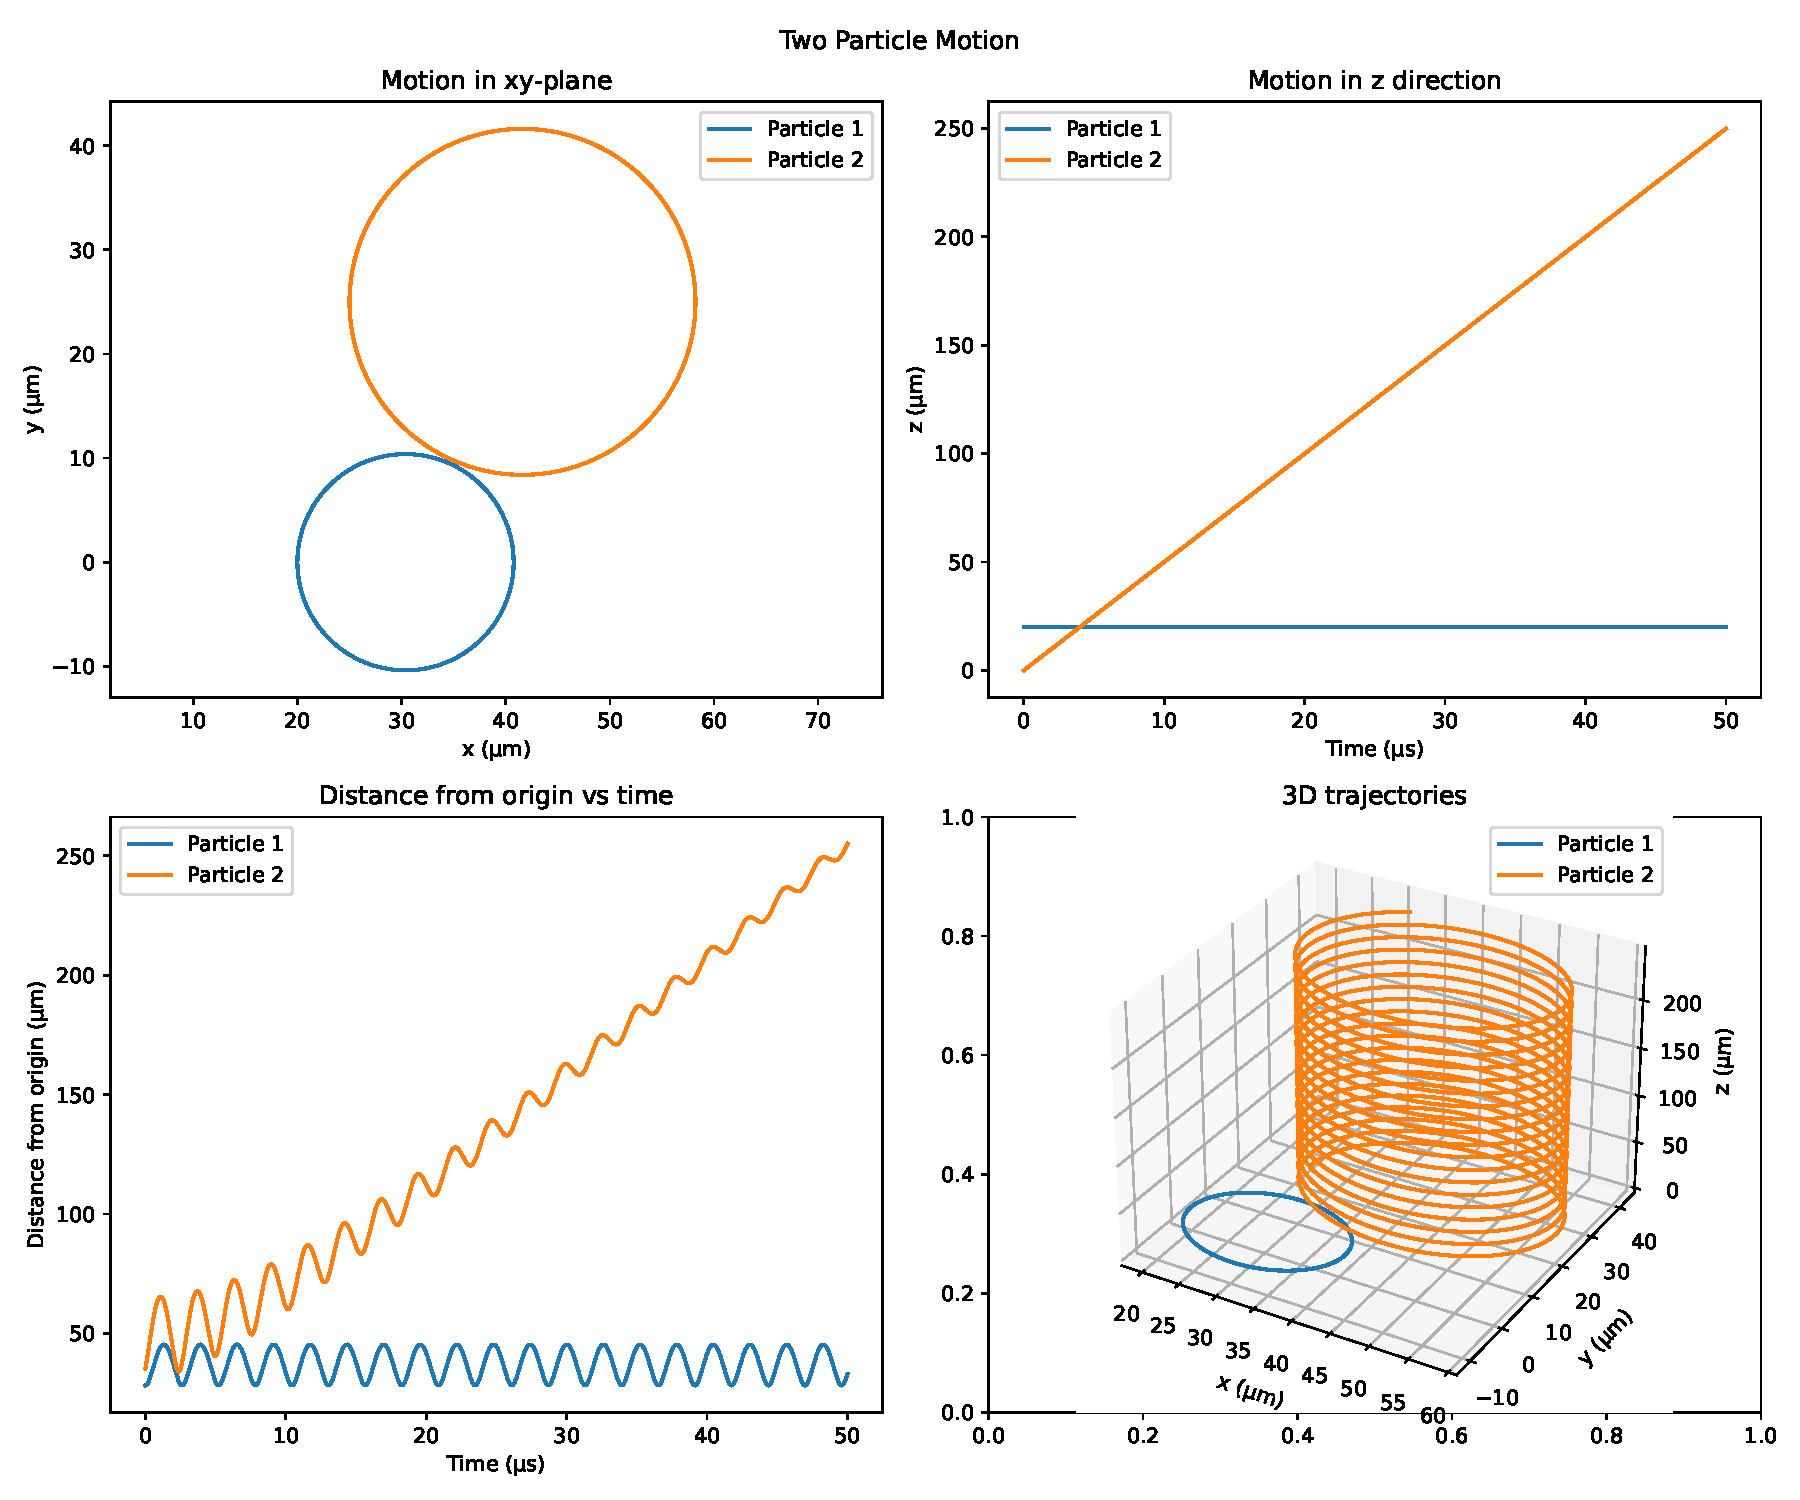
\includegraphics[width=0.48\textwidth]{build/figures/two_particles_motion_two_particles_without_interaction.pdf}
    \caption{Trajectories of two Ca$^+$ ions in the Penning trap without Coulomb interaction. The motion combines cyclotron orbits in the $xy$-plane with harmonic oscillation in the $z$-direction.}
    \label{fig:two_particles}
\end{figure}

\begin{figure}[h!]
    \centering
    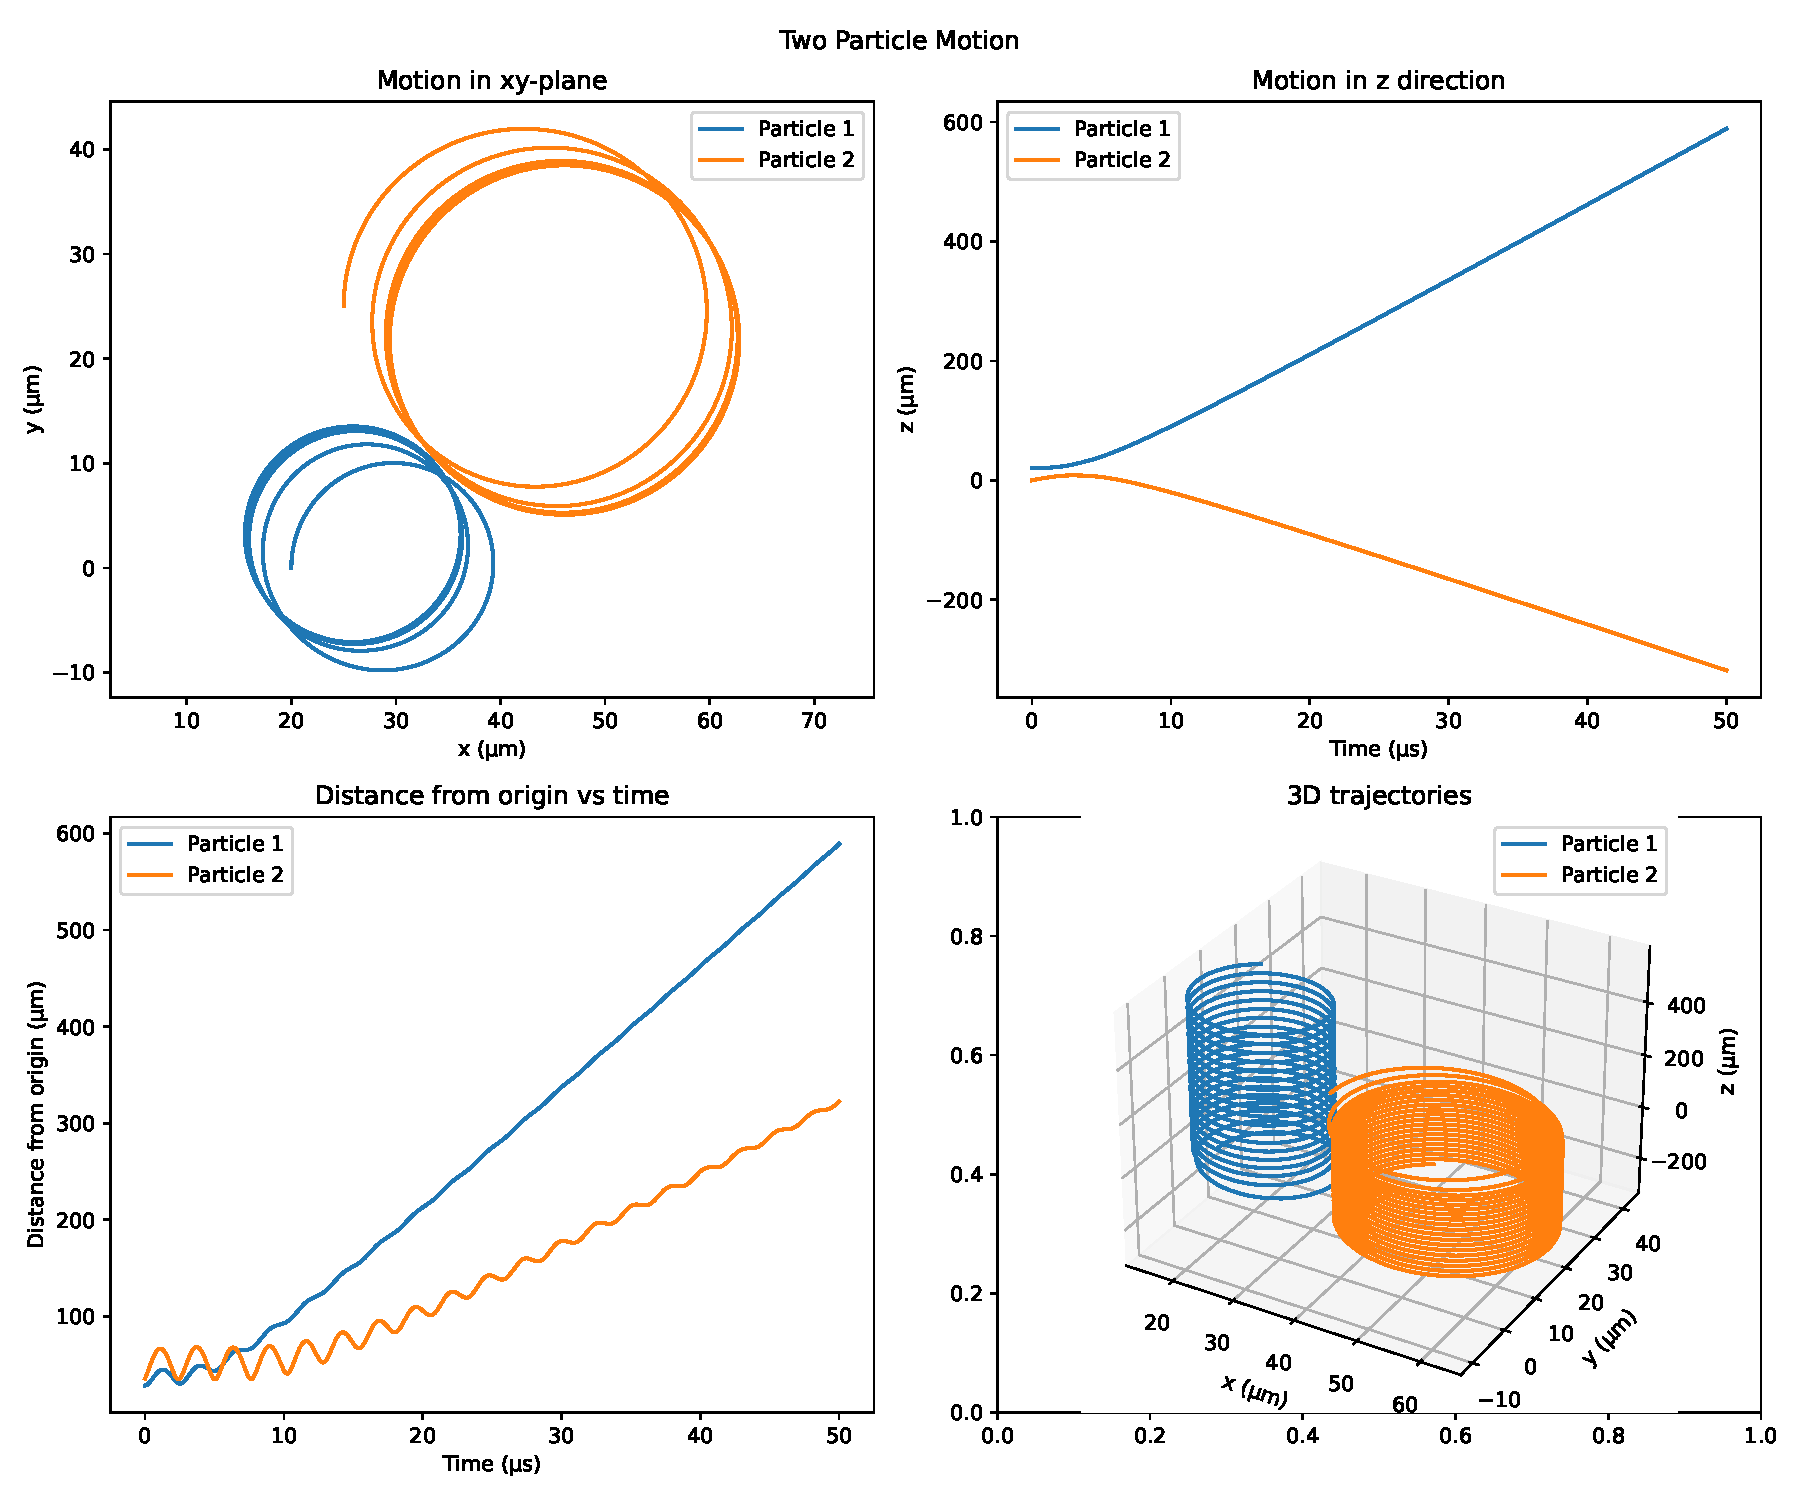
\includegraphics[width=0.5\textwidth]{build/figures/two_particles_motion_two_particles_with_interaction.pdf}
    \caption{Trajectories of two Ca$^+$ ions with Coulomb interaction enabled. The repulsive force between the particles modifies their orbits but does not destabilize the confinement.}
    \label{fig:two_particles_coulomb}
\end{figure}

Without Coulomb interactions (Figure \ref{fig:two_particles}), each particle follows an independent trajectory determined solely by the external electromagnetic fields. The motion combines cyclotron orbits in the $xy$-plane with harmonic oscillation in the $z$-direction. When Coulomb interactions are enabled (Figure \ref{fig:two_particles_coulomb}), we observe modified trajectories due to the mutual repulsion between the particles. Despite this additional force, both particles remain confined within the trap, demonstrating the robustness of the Penning trap's confinement mechanism.

\subsection{Resonance Analysis}

Our investigation of resonance phenomena reveals how the trap's confinement capabilities can be compromised by specific driving frequencies. Figure \ref{fig:resonance} shows the fraction of particles remaining in the trap after 500 $\mu$s of simulation time, for three different amplitudes of the time-varying potential.

\begin{figure}[h!]
    \centering
    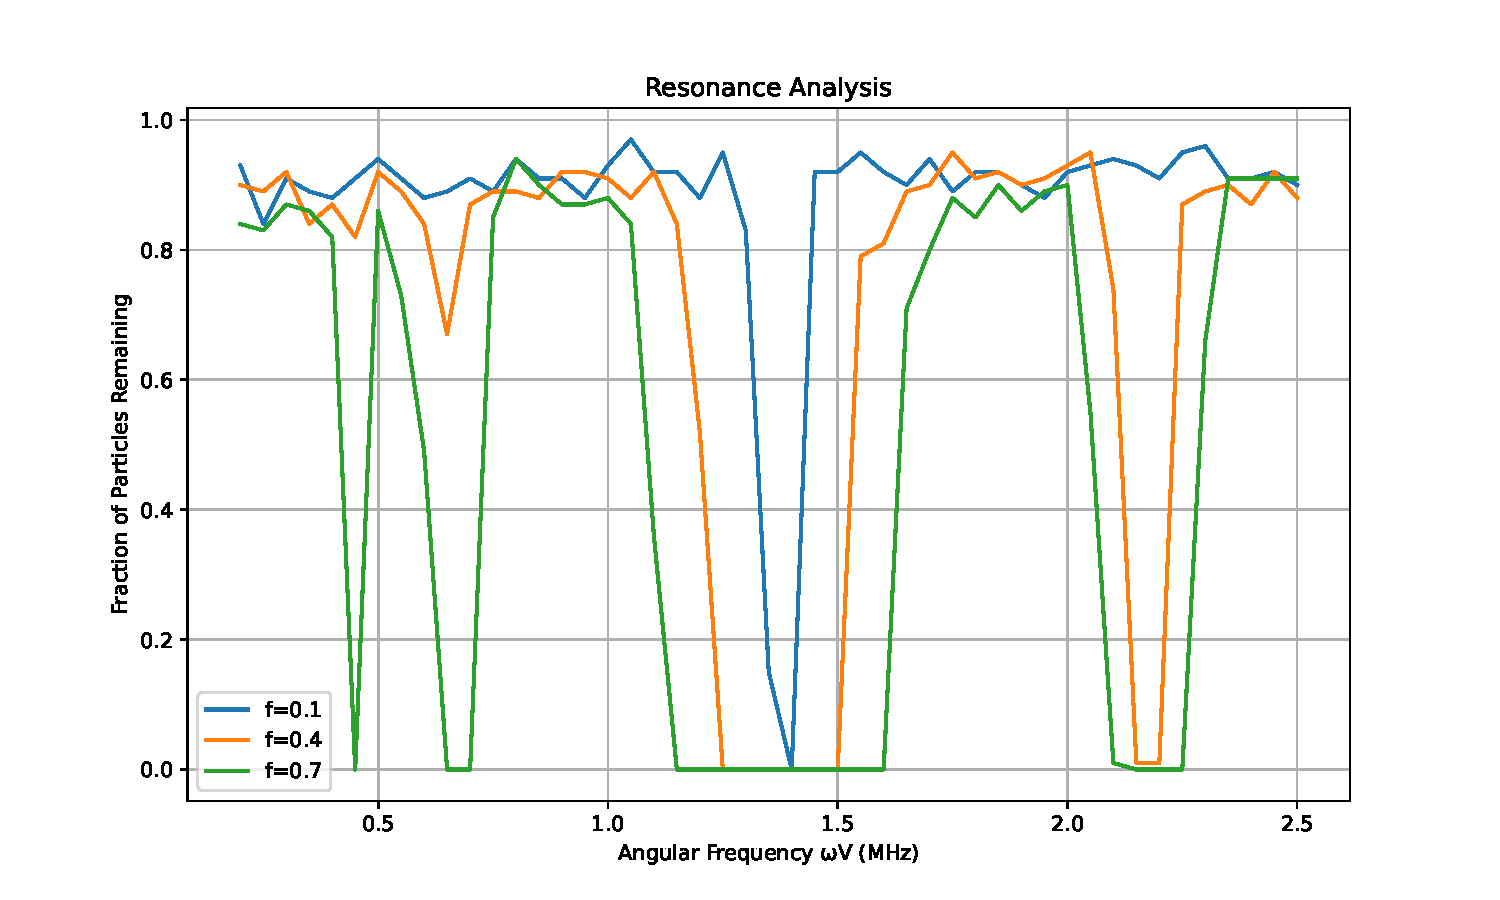
\includegraphics[width=0.5\textwidth]{build/figures/resonance_analysis.pdf}
    \caption{Fraction of particles remaining in the trap as a function of driving frequency $\omega_V$ for three different amplitudes $f$. Strong particle loss occurs at frequencies that are multiples of the axial frequency $\omega_z$.}
    \label{fig:resonance}
\end{figure}

Several key observations emerge from the resonance analysis:

1. Clear resonances appear at frequencies that are multiples of the axial frequency $\omega_z \approx 0.6936$ MHz.
2. The width of the resonance peaks increases with the amplitude $f$ of the time-varying potential.
3. Higher amplitudes lead to particle loss over a broader range of frequencies.

The fine-grained analysis around $\omega_V = 2\omega_z$ reveals subtle differences between systems with and without Coulomb interactions. When Coulomb interactions are present, the particle loss pattern becomes less sharp, suggesting that inter-particle forces can both enhance and inhibit the resonant ejection process.

These results demonstrate that while the Penning trap provides stable confinement under normal conditions, specific combinations of driving frequencies and amplitudes can lead to systematic particle loss. Understanding these resonance patterns is crucial for maintaining stable particle confinement in experimental settings.
\subsection{Error Analysis}

To validate our numerical methods, we conducted a detailed error analysis by comparing our numerical solutions with the analytical solution for a single particle. We simulated the system for 50 $\mu$s using four different time step sizes, corresponding to $n = 4000$, $8000$, $16000$, and $32000$ steps. Figure \ref{fig:error_analysis} shows the relative error evolution for both the Forward Euler and RK4 methods.

\begin{figure}[h!]
    \centering
    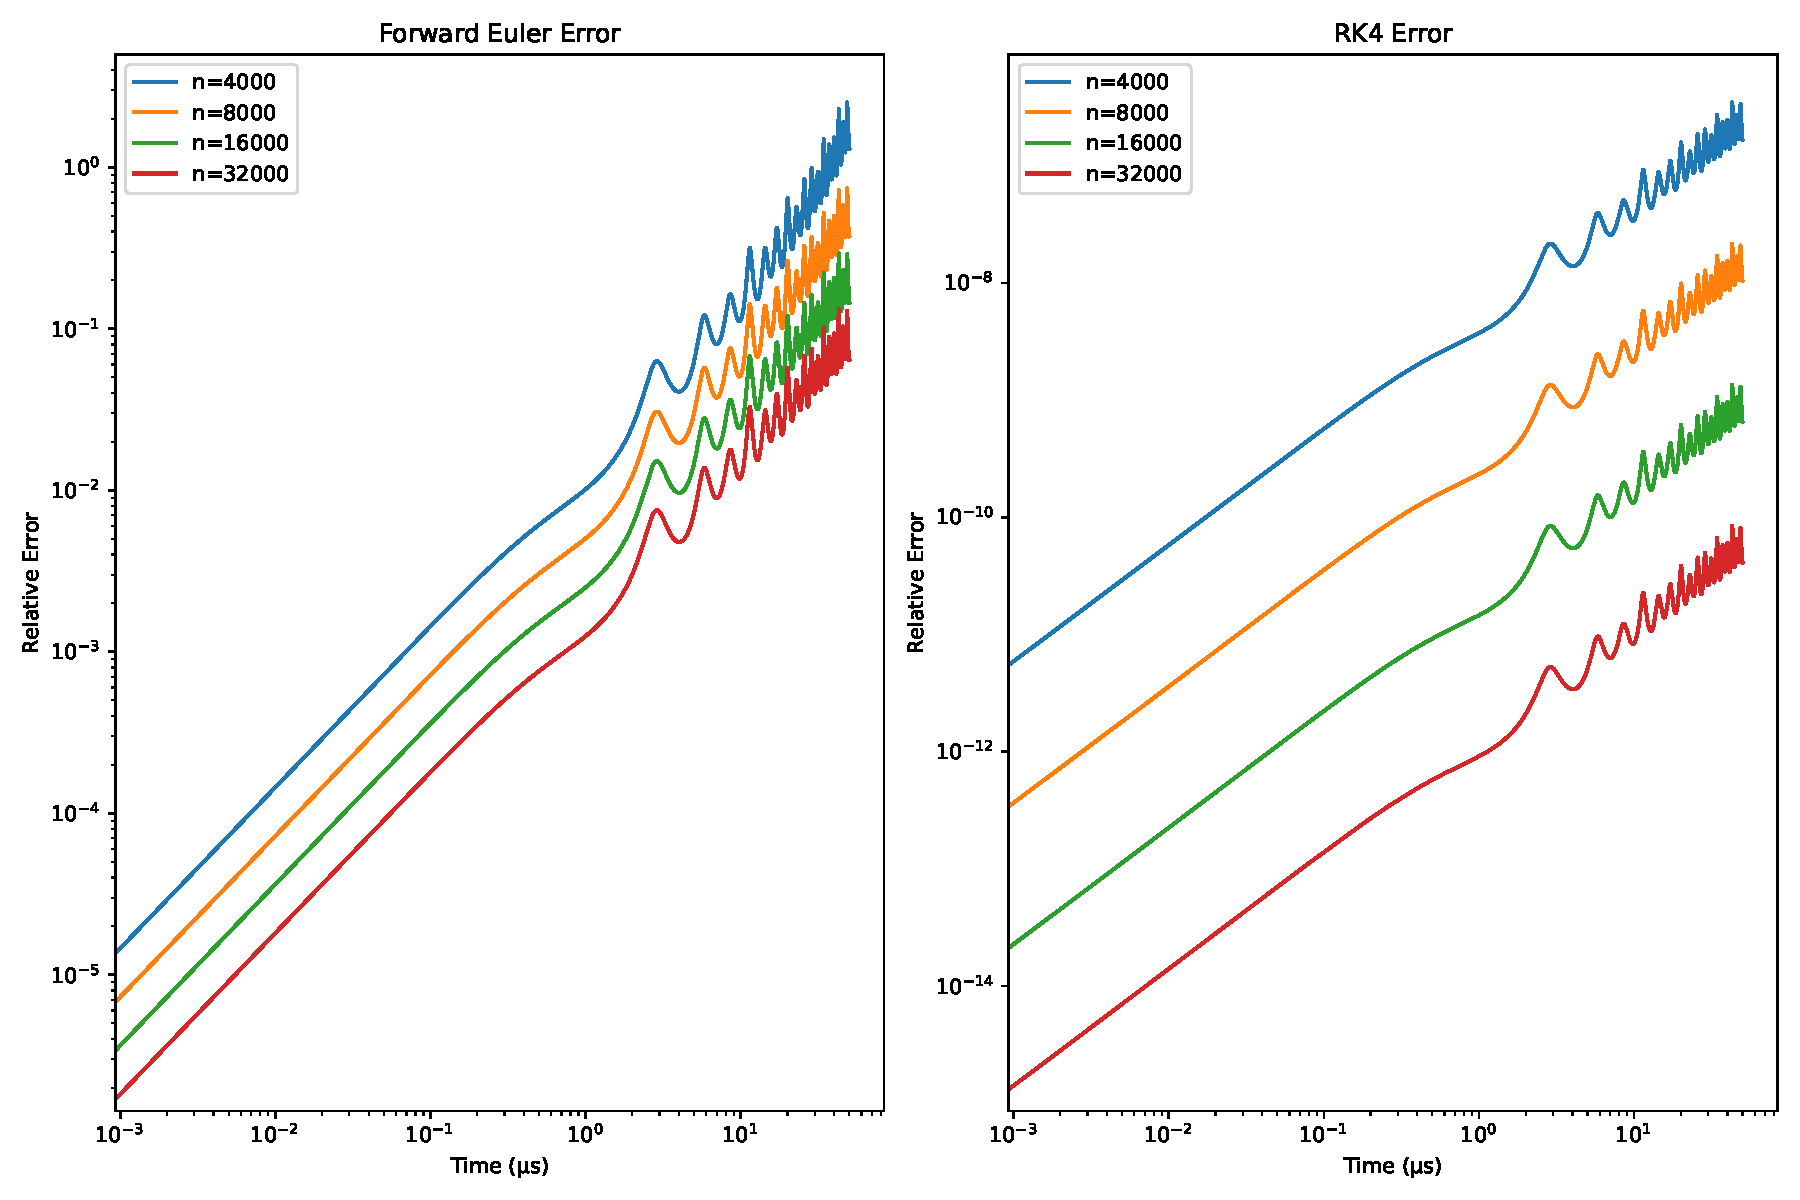
\includegraphics[width=0.48\textwidth]{build/figures/error_analysis.pdf}
    \caption{Relative error analysis for Forward Euler (left) and RK4 (right) methods with different numbers of time steps. The error is calculated relative to the analytical solution for a single particle's trajectory.}
    \label{fig:error_analysis}
\end{figure}

The Forward Euler method shows significantly larger errors compared to RK4, with relative errors typically several orders of magnitude higher. For the Forward Euler method, we obtained an error convergence rate of 1.46, while the RK4 method achieved a convergence rate of 1.27. Interestingly, while the Forward Euler method shows a faster convergence rate, its absolute error remains substantially larger than RK4 across all time step sizes.

This difference in accuracy is particularly evident when examining the particle's trajectory over longer time periods. The RK4 method maintains stable orbital patterns consistent with the analytical solution, while the Forward Euler method shows gradual deviation from the expected trajectory, especially in the xy-plane where the motion is more complex due to the coupling between x and y coordinates.

These results confirm the superior accuracy of the RK4 method for our Penning trap simulation, making it the preferred choice for our subsequent analyses of multi-particle systems and resonance phenomena.

% ===========================================
\section{Conclusion}\label{sec:conclusion}
%

We have successfully developed and validated a numerical simulation of a Penning trap for studying the dynamics of Ca$^+$ ions. Through comparison with analytical solutions, we demonstrated that our fourth-order Runge-Kutta implementation provides accurate particle trajectory predictions, significantly outperforming the Forward Euler method in terms of accuracy and stability over long simulation times.
Our investigation of two-particle dynamics revealed that while Coulomb interactions modify particle trajectories, they do not compromise the fundamental confinement mechanism of the trap. The addition of a time-dependent electric potential identified specific resonance frequencies, particularly at multiples of the axial frequency $\omega_z$, where particles are systematically ejected from the trap. The efficiency of this particle ejection increases with the amplitude of the time-varying potential, and the presence of Coulomb interactions tends to broaden these resonance features.
% ===========================================
% \section*{Appendix A}\label{sec:AppendixA}

% An appendix can be useful if there are details you want to include that do not fit in the main text. But if you include an appendix, make sure to explicitly refer to it somewhere in the main text.


% ===========================================
\onecolumngrid
% \bibliographystyle{apalike}
\bibliographystyle{unsrt}
\bibliography{ref}


\end{document}

\section{Problem 1}
The eq(15) is :
\begin{equation}
    \Ddot{z}+\omega_z^2z=0
\end{equation}
and it's a basic harmonic equation of which general solution is :
\begin{equation}
    z(t)=Acos(\omega_zt)+Bsin(\omega_zt)
\end{equation}
with A and B as constants and $\omega$ as angular frequency where $\omega_z = \sqrt{\frac{2qV_o}{md^2}}$.\\

\section{Problem 2}
We have to show that the two following equations can be rewritten as the third one with $f(t) = x(t) + iy(t)$.
\begin{equation}
    \Ddot{x}-\omega_0\dot{y}-\frac{1}{2}\omega_z^2x=0
\end{equation}
\begin{equation}
    \Ddot{y}+\omega_0\dot{x}-\frac{1}{2}\omega_z^2y=0
\end{equation}
\begin{equation}
    \Ddot{f}+i\omega_0\dot{f}-\frac{1}{2}\omega_z^2f=0
\end{equation}
First step : derivate $f(t) = x(t) + iy(t)$.
\begin{equation}
    \dot{f}(t) = \dot{x}(t) + i\dot{y}(t)
\end{equation}
\begin{equation}
    \Ddot{f}(t) = \Ddot{x}(t) + i\Ddot{y}(t)
\end{equation}
Second step : rewrite the eq(3) and eq(4) in function of $\Ddot{x}$ and $\Ddot{y}$.
\begin{equation}
    \Ddot{x} = \omega_0\dot{y}+\frac{1}{2}\omega_z^2x
\end{equation}
\begin{equation}
    \Ddot{y}=-\omega_0\dot{x}+\frac{1}{2}\omega_z^2y
\end{equation}
Third step : add eq(8) to the multiplication of i by eq(9) and simplify.
\begin{equation}
    \Ddot{x}+i\Ddot{y}=\omega_0(\dot{y}-i\dot{x})+\frac{1}{2}\omega_z^2(x+iy)
\end{equation}
\begin{equation}
    \Ddot{f}=-i\omega_0\dot{f}+\frac{1}{2}\omega_z^2f
\end{equation}
So we found :
\begin{equation}
    \Ddot{f}+i\omega_0\dot{f}-\frac{1}{2}\omega_z^2f = 0
\end{equation}

\section{Problem 3}
ok,hmm\\
here answers for problem 3 : we just have to have $\omega_0^2 \geq 2\omega_z^2$\\
with $\omega_0=\frac{qB_0}{m}$ and $\omega_z^2=\frac{2qV_0}{md^2}$ we just have to have $B_0^2 \geq \frac{2V_0}{d^2}$.

\section{Problem 4}
Retake the eq(17), $r(t)=\abs{f(t)}$, $(\abs{z_1+z_2})^2=\abs{z_1}^2+\abs{z_2}^2+2Re(z_1*z_2)$, cos oscillate between 1 and -1, so R+ is when cos(...)=1 and R- is when cos(...)=-1, then we refind R+ and R-.

